%{\bf Add information about the vertical slice at CERN and eventual
%test beam studies}

In order to integrate the various components of the NSW electronics,
a vertical slice of the system will be assembled in a lab on the Meyrin site.
It will include prototypes of all components from VMMs through the Trigger Processors, ROD and an evaluation board to capture the Sector Logic input.
The slice can be used to playback captured and simulated data, injected at various points.
Unlike beam and cosmic ray tests, it will allow testing the Trigger Processors at the 40\,MHz bunch crossing rate.

Part of the testing strategy for the Micromegas trigger includes
the installation of the Micromegas Small Wheel (MSW) in the ATLAS
cavern.
This will allow the Micromegas trigger to be tested with low-level cavern background conditions.
The electronics chain for the MSW will
include the VMM2 readout chip and the ADDC card for transmitting ART
signals to an evaluation board located in USA15. The evaluation board
will receive the ART signals from the ADDC and decode them. On an
ATLAS Level-1 Accept, the evaluation board will format all of the ART
data within four bunch crossings of the ATLAS trigger and send them to
the ATLAS DAQ system via ethernet. Events will also be sent via a second ethernet
link to a desktop PC to allow for real time monitoring. Recording the
data in this way will allow for testing of the trigger algorithm and
implementation using ART data from Micromegas with some cavern background.
The trigger algorithm for segment reconstruction can be implemented in the evalaution board and recorded.
The collected ART data can also later be replayed through existing pattern
generators to allow for quick debugging of the trigger electronics,
offering a set of tests different from those generated by Athena.
Figure\,\ref{fig:MSWChain} shows the trigger chain envisioned for the MSW.

\begin{figure}[h!]
 \centering
 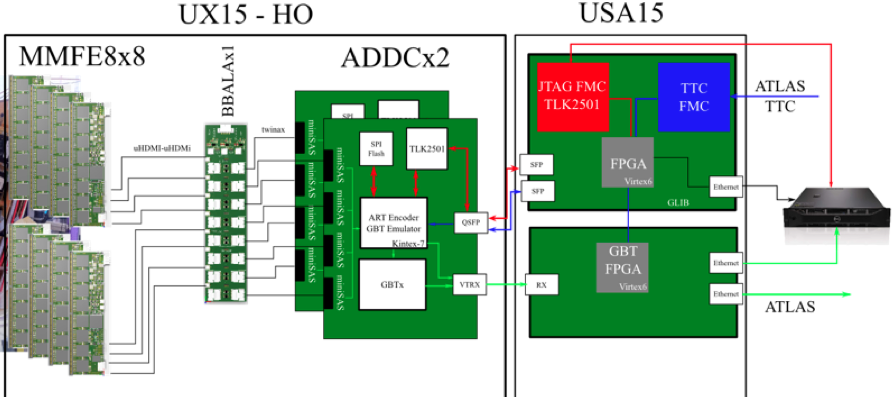
\includegraphics[width=0.9\textwidth]{figures/MSW_Trigger}
 \caption{MSW trigger chain proposal}
 \label{fig:MSWChain}
 \end{figure}


\FloatBarrier